\documentclass{article}

\usepackage{amsmath}
\usepackage{graphicx}

\begin{document}

\section{Pressure Poisson Solver}

We have put our equations into a form such that for us to find the pressure
	within the cavity, we need to solve a poisson equation,
	with source terms that we have determined.
We will first exhibit the Gauss-Seidel approach, and summarize its characteristics
	and drawbacks.
We will then investigate the multigrid approach.

\subsection{Gauss Seidel}

Gauss-Seidel iteration splits up our linear operator laplacian $A$ into
	an upper triangular and lower triangular part, $L$ and $U$,
	such that $A = L + U$, and $L$ contains the diagonal elements.
A linear equation is now of the form:

\begin{align}
A x = b \\
(L + U) x = b\\
L x = b - U x
\end{align}

For the iteration, we let the $k+1$-st iteration be:

\begin{align}
L x^{(k+1)} = b - U x^{(k)}
\end{align}

From Matrix Computations, by Golub and Van Loan, this can be expressed as:

\begin{align}
x_l^{(k+1)} & = \frac{1}{a_{ll}} \left( b_l 
	- \sum_{l=1}^{i-1} a_{lm} x_m^{(k+1)}
	- \sum_{l=i+1}^n a_{lm} x_m^{(k)} \right)
\end{align}

If we are using a rasterized grid, then the terms in the first
	sum will only be nonzero for the neighbors to the left
	and below the current node,
	while the terms in the second sum will only be nonzero for
	the neighbors to the top and right of the current node.
Assuming that $dx = dy = \Delta$, their coefficients will all be $1/\Delta^2$.
Also, $a_{ll}$, the current coefficient, will be $\frac{-4}{\Delta^2}$.

Thus, we can rewrite the sum as follows:

\begin{align}
x_{i,j}^{(k+1)} & = - \frac{\Delta^2}{4} \left( b_{i,j} 
	- \frac{1}{\Delta^2} x_{i,j-1}^{(k+1)}
	- \frac{1}{\Delta^2} x_{i-1,j}^{(k+1)}
	- \frac{1}{\Delta^2} x_{i+1,j}^{(k)}
	- \frac{1}{\Delta^2} x_{i,j+1}^{(k)} \right)\\
x_{i,j}^{(k+1)} & = \frac{1}{4} \left(
	x_{i,j-1}^{(k+1)}
	+ x_{i-1,j}^{(k+1)}
	+ x_{i+1,j}^{(k)}
	+ x_{i,j+1}^{(k)}
	- \Delta^2 b_{i,j} \right)
\end{align}

Note that if we are iterating through all of the interior nodes,
	all of the nodes before the current one will have been updated,
	and all of the nodes after the current one will not have been.
Therefore, we can use this algorithm \emph{in-place} on an array,
	a very desirable property.

\subsubsection{Testing Gauss-Seidel}

I implemented a basic version of Gauss-Seidel from a problem that I got from
	a powerpoint by Xiao-Ping Wang, of Hong Kong University of Science
	and Technology.
It contanins the following differential equation source term, and analytical solution:

\begin{align}
	\nabla^2 u(x,y) & = -2 \left[ (1 - 6 x^2) y^2 (1-y^2) + (1-6y^2)x^2(1-x^2) \right]\\
	u(x,y) & = (x^2 - x^4)(y^4-y^2)
\end{align}

We found that we were able to achieve convergence with the Gauss-Seidel iteration,
	starting from an initial guess of zero,
	but the speed of convergence depended very strongly on the size of the grid.
Smaller grids produced convergance much more quickly.

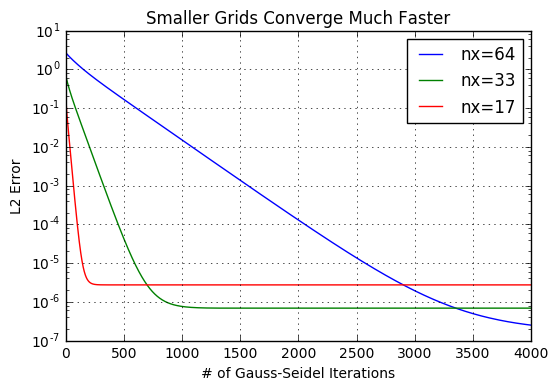
\includegraphics[width=\textwidth]{gauss-seidel-error-decreasing}

It would be very useful to be able to exploit the rapid convergence properties
	of coarse grids while still being able to use a fine solution,
	which we will attempt to do with multigrid methods.

\end{document}
